\documentclass[12pt,a4paper]{article}
\usepackage[utf8]{inputenc}
\usepackage[T1]{fontenc}
\usepackage{titling}
\usepackage{amsfonts}
\usepackage{amssymb}
\usepackage{tcolorbox}
\usepackage{mdframed}
\usepackage{graphicx}
\usepackage{wrapfig}
\usepackage{libertine}

\usepackage{amsfonts}
\usepackage[top=1in, bottom=1.5in, left=1in, right=1in]{geometry}
\renewcommand{\contentsname}{Sadržaj}

\setlength{\droptitle}{-8em}

\title{\Large \textsc{univerzitet u novom sadu
\\prirodno-matematički fakultet
\\departman za
\\matematiku i informatiku}
\vspace{5em} 
\\ \textbf{Remzijevi brojevi}
\vspace{1em} }


\graphicspath{ {/hdd/seminarski/GeogebraSlike//} }

\begin{document}
		
	\author{
  	Renea Mošo\\
  	\texttt{}
  	\and
  	Nikola Obradović\\
  	\texttt{}
  	\and
  	Nikola Pešić
	}	
	\date{}
	
	\maketitle
	
	\thispagestyle{empty}
	
	\newpage
	
	\tableofcontents
	\newpage
	
	\section{Uvod u Remzijevu teoriju}
	Obrad
	\newpage
	
	
	\section{Remzijevi brojevi}
	\vspace{1em}
	{\fontsize{12pt}{12pt}\textbf{Definicija}}
	\vspace{0.5em}	
	\\
	Remzijev broj $R(l_{1}, l_{2})$ je najmanje $n \in \mathbb{N}$ \textbackslash {} 0 takvo da $n\rightarrow(l_{1}, l_{2})$.
	
	
	\vspace{1em}
	{\noindent\fontsize{12pt}{12pt}\textbf{Primer}}
	\vspace{0.5em}
	\\	
	Pronađimo $R(3,3)$ :
	\\Počnimo od broja 6. Dokazaćemo da je $6 \rightarrow (3, 3)$. Uočimo čvor A. Po Dirihleovom principu bar 3 od 5 veza čvora A sa ostalim čvorovima mora biti obojeno istom bojom. 
	\begin{figure}[h]
	\centering
	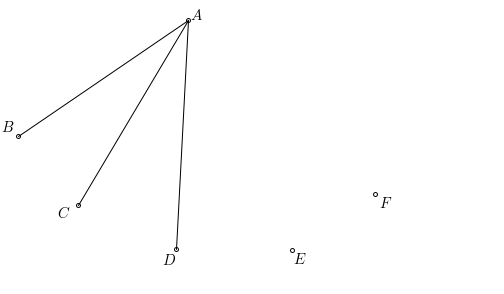
\includegraphics[scale=2.3]{r33.png}
	\end{figure}
	
	\noindent Na slici su grane jedne boje obojene u crno, dok su ostale bele (ne vide se).
	Neka su, bez umanjenja opštosti, grane čvora A koje su incidentne sa čvorovima B, C i D obojene istom bojom (crnom). Sada postoje dve mogućnosti: 
	\vspace{1em}
	\\
	$1^\circ$ Sve grane koje povezuju čvorove B, C i D su obojene belom bojom Tada čvorovi B, C, i D obrazuju kompletan graf reda 3 obojen belom bojom.
	\vspace{0.5em}
	\\
	$2^\circ$ Bar jedna od grana koje povezuju čvorove B, C i D je obojena crnom bojom. Bez umanjenja opštosti, neka je to grana koja povezuje B i C. Tada čvorovi A, B i C sačinjavaju kompletan graf reda 3 obojen crnom bojom.
	\vspace{0.5em}
	\\Dokazali smo da je $6 \rightarrow (3, 3)$, a sada još treba dokazati da ne važi $5 \rightarrow (3, 3)$. Za to je dovoljno da pronađemo kontra primer bojenja u kojem uslov nije ispunjen:
	\begin{figure}[h]
	\centering
	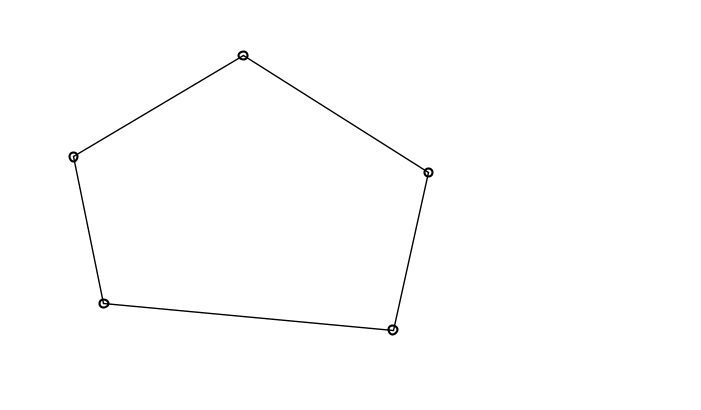
\includegraphics[scale=1.3]{r33kp.png}
	\end{figure}
	
	Dakle, $R(3,3)=6$ .
	
	\newpage
	
	
	\section{Granice remzijevih brojeva}
	Pesic
\end{document}